\documentclass[letterpaper]{article} % DO NOT CHANGE THIS
\usepackage[submission]{aaai2027}  % DO NOT CHANGE THIS
\usepackage[hyphens]{url}  % DO NOT CHANGE THIS
\usepackage{graphicx} % DO NOT CHANGE THIS
\urlstyle{rm} % DO NOT CHANGE THIS
\def\UrlFont{\rm}  % DO NOT CHANGE THIS
\usepackage{natbib}  % DO NOT CHANGE THIS AND DO NOT ADD ANY OPTIONS TO IT
\usepackage{caption} % DO NOT CHANGE THIS AND DO NOT ADD ANY OPTIONS TO IT
\frenchspacing  % DO NOT CHANGE THIS
\usepackage{algorithm}
\usepackage{algorithmic}
\usepackage{booktabs}
\usepackage{amsmath}
\usepackage{amsthm}
\pdfinfo{
/TemplateVersion (2027.1)
}

\newtheorem{proposition}{Proposition}

\newcommand{\mcold}{\textsc{Cold}}
\newcommand{\mhint}{\textsc{Hint}}
\newcommand{\mfloor}{\textsc{Floor}}
\newcommand{\mfh}{\textsc{Floor+Hint}}
\newcommand{\mrho}{\textsc{RepHint}}
\newcommand{\mspt}{\textsc{SPT+Cold}}
\newcommand{\mmwkr}{\textsc{MWKR+Cold}}
\newcommand{\miaip}{\textsc{IAIP-SR}}
\newcommand{\melr}{\textsc{ELR}}
\newcommand{\mfresh}{\textsc{Fresh+Cold}}
\newcommand{\mfreshh}{\textsc{Fresh+Hint}}
\newcommand{\mpc}{\textsc{Port+Cold}}
\newcommand{\mph}{\textsc{Port+Hint}}
\newcommand{\mrnd}{\textsc{Random-N}}
\newcommand{\melrc}{\textsc{ELR+Cold}}

\setcounter{secnumdepth}{0}

\title{Reuse, Then Focus: Incumbent Portfolios and Impact-Selective CP-SAT\\for Anytime Rescheduling}
\author{
    Anonymous Submission
}
\affiliations{
}

\begin{document}

\maketitle

\begin{abstract}
When a job shop changes---a job arrives, a machine fails---the schedule is recomputed under a tight time budget. We study how the previous schedule should be used by a constraint solver in this setting, measuring anytime quality by the primal integral with streams, not instances, as the unit of inference. First, with five solver seeds on 45 streams, keeping a repaired copy of the previous schedule as an incumbent beside an unmodified CP-SAT run (a \emph{floor}) beats both solving from scratch and the stronger baseline of starting from a fresh dispatching-rule schedule, whereas passing the previous or repaired schedule as a solver hint is worse than not reusing it. The floor fails after job arrivals. Second, we combine three known ingredients---a portfolio of historical and fresh incumbents including an event-localized insertion repair, a restricted CP-SAT solve on a bounded neighbourhood of the operations the event affected, and a hinted unrestricted continuation---under a single wall-clock deadline. On 40 held-out streams, under a configuration frozen on separate development streams, this reduced the primal integral by 43\% relative to the best fresh-incumbent baseline, on every stream, and improved the final gap; ablations attribute the gain to all three components, and an impact-aware neighbourhood beat a random one of the same size. In exploratory experiments the reduction held, and grew, with 30\,s budgets, four solver workers, arrival-only, outage-only and high-severity streams and 34 published base instances, although the restricted stage's own contribution was not detectable with 2\,s budgets or four workers.
\end{abstract}

\section{Introduction}

Schedules in manufacturing are revised repeatedly as jobs arrive, durations change and machines fail, and each revision must be produced within a time limit set by operations \citep{vieira2003,ouelhadj2009}. Planning research has long asked whether to repair the previous plan or plan anew \citep{nebel1995,vanderkrogt2005,fox2006}, and rescheduling research has asked how much of a schedule to reoptimize after a disruption, from right-shifting to affected-operations rescheduling to full regeneration \citep{abumaizar1997,subramaniam2003,sun2026}. With a modern constraint solver, both questions become questions about \emph{how the previous schedule enters the solve}, and about \emph{where in the budget} effort goes.

The common answer is a solver \emph{hint} (warm start). We find it unreliable, and we find a simpler alternative reliable: repair the previous schedule constructively and keep it as an incumbent---a floor---beside an unmodified solver run. A floor costs no search effort, but it is only as good as the repair. After a job arrival, appending the new job to the old schedule produces a poor incumbent, and then a schedule built from scratch by a dispatching rule is better.

This paper makes two empirical contributions, with a protocol designed to avoid the inflated significance of instance-level tests: streams are the unit of inference, every method uses five solver seeds, and the main method's configuration was frozen on development streams before it was run on held-out ones.
\begin{itemize}
\item \textbf{Historical reuse versus fresh construction.} On 45 job-shop streams, \mfloor{} beats solving from scratch by 23.6\% in primal integral and beats CP-SAT started from an MWKR or SPT schedule by 15.8\% and 16.9\%, winning on 44--45 of 45 streams (41--45 under a second reuse protocol). Every hint-based variant is worse than its hint-free counterpart.
\item \textbf{A budget-shared pipeline} (\miaip) that keeps the best of several historical and fresh incumbents, spends up to 60\% of the budget optimizing a neighbourhood around the operations affected by the event with all other machine orders fixed, and continues with the unrestricted solver. On 40 held-out streams it reduces the primal integral by 43.2\% against the strongest fresh-incumbent baseline (40/40 streams) and by 36.1\% against \mfloor{}. Ablations attribute the gain to history-based incumbents, to the hinted continuation, and to the restricted stage, and show that an impact-aware neighbourhood beats a random one of the same size. Exploratory experiments with other budgets, worker counts, delta mixes and published base instances confirm the overall reduction and delimit when the restricted stage itself matters.
\end{itemize}
None of the three ingredients is new: affected-operations rescheduling \citep{abumaizar1997}, insertion into machine sequences \citep{werner1995}, large neighbourhood search with constraint programming \citep{shaw1998,godard2005}, and algorithm portfolios \citep{gomes2001} are well established. What we contribute is the evaluation of how to combine them under one anytime deadline against fresh-incumbent baselines, and the finding that the same solver hint that hurts when it comes from the previous schedule helps when it comes from the current incumbent.

\section{Related Work}

\paragraph{Rescheduling scope.} Affected Operations Rescheduling (AOR) reschedules only the operations a disruption affects and was compared with total and right-shift rescheduling \citep{abumaizar1997}; mAOR extends it to further disruption types \citep{subramaniam2003}. \citet{sun2026} study the optimization scope in dynamic flexible job shops---from minimal repair to global reoptimization---and its effect on quality and stability. Match-up scheduling reconstructs the schedule until it rejoins the original \citep{bean1991}. These works compare scopes by final quality and stability; we compare reuse strategies by the quality available throughout a fixed budget and against baselines that start from a fresh constructive schedule.

\paragraph{Repair and insertion.} Inserting operations one at a time into fixed machine sequences is a classical job-shop construction principle \citep{werner1995}; critical paths and blocks underlie the standard neighbourhoods \citep{vanlaarhoven1992,nowicki1996}. Plan repair and plan stability are studied in planning \citep{nebel1995,vanderkrogt2005,fox2006}, and solution reuse in dynamic constraint satisfaction \citep{verfaillie1994}.

\paragraph{Neighbourhood search with solvers.} Large neighbourhood search (LNS) relaxes part of an incumbent and re-solves it with constraint programming \citep{shaw1998}, including for cumulative and flexible job-shop scheduling \citep{godard2005,pacino2011}; local branching restricts a MIP to a neighbourhood of an incumbent \citep{fischetti2003}, and BALANS selects LNS operators online \citep{cai2025}. Our restricted stage is a single LNS step whose neighbourhood is chosen from the event, not by search. Warm-starting solvers after small data changes was the subject of a recent MIP computational competition \citep{bolusani2024}.

\paragraph{Portfolios and anytime evaluation.} Keeping the best of several constructive starts is GRASP-like multi-start \citep{feo1995} and an algorithm portfolio \citep{gomes2001}. Anytime algorithms trade quality for time \citep{dean1988,zilberstein1996}; we measure this trade-off with the primal integral \citep{berthold2013}.

\section{Problem Setting}

A \emph{stream} is a sequence of job-shop instances $I_0,\dots,I_T$ in which $I_t$ arises from $I_{t-1}$ by a \emph{delta}: a job arrival, a job cancellation, a change of one job's durations, or an outage window on one machine. Each instance is solved within a wall-clock budget $B$, covering construction, model building, solving and validation. A method receives $I_t$ and the solution it returned for $I_{t-1}$. The objective is the makespan.

For a run on $I_t$, $z(\tau)$ is the makespan of the best schedule found by time $\tau$. Let $z^*$ be the best makespan found for $I_t$ by any run of any method in the same experiment. With gap $g(\tau)=(z(\tau)-z^*)/z^*$, and $g(\tau)=1$ before the first schedule, the primal integral is $\mathrm{PI}=\frac{1}{B}\int_0^B g(\tau)\,d\tau$; lower is better. Schedules found after $B$ are ignored.

\paragraph{Unit of inference.} Steps of a stream share their history, and solver seeds share their instance, so neither is an independent observation. We average PI over solver seeds and over steps $1,\dots,T$ within each stream and compare methods by paired stream-level differences: an exact two-sided sign test over streams, Holm correction within each predeclared family, and a 95\% bootstrap confidence interval that resamples streams (10{,}000 resamples).

\section{Methods}

\paragraph{Floor.} A repair $\rho(I_t,S_{t-1})$ orders surviving operations by their previous start, appends the operations of new jobs, and schedules each at its earliest feasible time, skipping machine outages. \mfloor{} records this schedule as soon as it is built and then runs CP-SAT on $I_t$ unhinted, with the same parameters and seed as solving from scratch (\mcold); the reported incumbent is the better of the two at every moment.

\paragraph{Event-localized repair (\melr).} Arrivals break the floor because appended operations ignore idle time and machine contention. \melr{} keeps the previous machine orders of surviving operations and re-inserts the operations the event introduced, and after an outage the operations the outage delays, job by job in decreasing total processing time, each at the position of its machine sequence that minimizes the estimated makespan through it \citep{werner1995}. Positions that would create a cycle with the operation's job predecessor or successor, or that precede a committed operation, are excluded; an allowed position always exists. The final schedule is the earliest-start schedule of the resulting orders, computed with machine outages, and is validated; any failure falls back to a dispatching rule that respects commitments. For cancellations and duration changes \melr{} coincides with the floor.

\paragraph{Incumbent portfolio.} The portfolio builds, in order, the floor, \melr, MWKR, SPT, a regret-based insertion variant of the floor, LPT and FIFO schedules, validates each, and publishes every member that improves on the best so far at the moment it is built (an anytime portfolio). Members that would exceed 5\% of $B$ are skipped. The \emph{fresh} portfolio contains only the four dispatching rules and never reads the previous schedule. It is our main baseline because, in contrast to \mcold{}, it isolates the value of history from the value of having any early incumbent.

\paragraph{Impact-selective CP-SAT.} Let $D$ be the operations whose inputs changed: new operations, operations with a changed duration, release date or commitment, the surviving machine successors of cancelled operations, and operations whose previous interval meets a new outage. The neighbourhood $N$ is a breadth-first expansion from $D$ over job and machine adjacency in the current incumbent $S$, capped at 25\% of all operations. The restricted model is the full CP-SAT interval model plus, for every machine and every pair $u,v\notin N$ consecutive in $S$'s machine order restricted to operations outside $N$, the precedence $s_v \ge s_u + p_u$, plus $C_{\max}\le C_{\max}(S)-1$. Operations in $N$ can move and be resequenced; the rest keep their relative order but can shift in time. The model is hinted with $S$.

\begin{proposition}
$S$ satisfies the added precedences, so the restricted problem without the improvement constraint contains $S$. With it, an INFEASIBLE status proves that no schedule better than $S$ preserves the machine orders outside $N$.
\end{proposition}
\begin{proof}
If $u$ precedes $v$ on a machine in $S$, then $s_u+p_u\le s_v$ because $S$ is feasible; the added constraints are a subset of these. The second claim is the definition of the added bound.
\end{proof}

\paragraph{\miaip.} Algorithm~\ref{alg:iaip} runs the three stages under one deadline. The restricted solve runs until $\alpha B$ elapsed, or until it proves optimality or infeasibility within the neighbourhood; the unrestricted CP-SAT run then continues, hinted with the current incumbent, until $B$. Every schedule is validated before it replaces the incumbent, and only strict improvements are accepted. The returned schedule is never worse than the best incumbent seen within the run; it is \emph{not} guaranteed to beat an independent \mcold{} run, because the first two stages take time away from it.

\begin{algorithm}[tb]
\caption{\miaip{} under a single deadline $B$}
\label{alg:iaip}
\textbf{Input}: $I_{t-1}$, $S_{t-1}$, $I_t$, budget $B$, share $\alpha$\hfill\\
\textbf{Output}: validated schedule, trajectory
\begin{algorithmic}[1]
\STATE start the clock; $D\leftarrow$ disrupted operations of $I_t$
\STATE build the portfolio; publish each improving member when built
\STATE $N\leftarrow$ bounded expansion of $D$ around incumbent $S$
\STATE restricted CP-SAT on $N$ (orders outside $N$ fixed, $C_{\max}<C_{\max}(S)$, hint $S$) until $\alpha B$; keep validated improvements
\STATE unrestricted CP-SAT hinted with the current incumbent until $B$; keep validated improvements
\STATE \textbf{return} the incumbent
\end{algorithmic}
\end{algorithm}

\section{Experimental Protocol}

\paragraph{Streams and solver.} Base instances are full $m{\times}m$ job shops with durations uniform in $[5,50]$; deltas are drawn with weights 0.4 (arrival), 0.2 (cancellation), 0.25 (duration jitter) and 0.15 (outage), ten per stream. CP-SAT (OR-Tools 9.15) runs with one worker, $B=8$\,s. Each process is pinned to its own physical core of an Intel Core i7-12700 (P-cores only for all reported confirmatory and Stage~1 runs), and the order of methods within a step is shuffled. Every returned schedule is checked by an independent validator.

\paragraph{Stage 1: historical reuse.} Seven methods on 45 streams ($m\in\{10,15,20\}$, 15 stream seeds) and solver seeds 0--4: \mcold, \mhint{} (previous solution as hint), \mfloor, \mfh{} (floor plus the floor as hint), \mrho{} (the floor as hint, not retained), \mspt{} and \mmwkr{} (dispatching schedule retained as incumbent, then unhinted CP-SAT). Under Protocol~B each method carries its own previous solution; under Protocol~A the history-based methods receive a common previous solution from a reference chain. The design and decision rule were written down before results were inspected.

\paragraph{Stage 2: development and freeze.} Portfolio composition, neighbourhood type (disruption set, forward closure, critical path, their union, bounded expansion, random), budget share $\alpha$ and continuation mode (unhinted, hinted, cutoff) were chosen on separate development streams (stream seeds 301--310, never used for confirmation). The chosen configuration---full portfolio, bounded expansion at 25\%, $\alpha=0.6$, hinted continuation---was written to a configuration file with its SHA-256 hash before the confirmatory run, together with the comparators, the eight-member comparison family and the success criteria; the analysis script refuses to run if the file has changed. Three deviations from the original pre-registration, all made before any confirmatory run, are recorded: the portfolio was made anytime after development showed that waiting for all members cost more than they recovered, which strengthens the fresh baseline; since the frozen continuation is hinted, the control for the restricted stage became \mph{} instead of \mpc; and three comparators (\mfreshh, \mrnd, \mpc{} vs \mfresh) were added, enlarging the family from five to eight.

\paragraph{Stage 3: confirmation.} Ten methods on 40 held-out streams ($m\in\{15,20\}$, stream seeds never used before), solver seeds 0--4: \miaip; \mph{} (portfolio and hinted continuation, no restricted stage); \mpc{} (portfolio, unhinted); \mfresh{} and \mfreshh{} (fresh portfolio, unhinted or hinted); \mmwkr; \mfloor; \mcold; \melrc; and \mrnd{} (\miaip{} with a random neighbourhood of the same size).

\section{Results}

\paragraph{Integrity.} All 26{,}325 Stage~1 runs and 22{,}000 confirmatory runs returned a validated schedule. Runs ended at most 0.18\,s (Stage~1) and 0.24\,s (confirmatory) after the deadline, the 99th percentile being 0.016--0.017\,s; these runs are kept, and incumbents after $B$ are ignored.

\paragraph{Historical reuse beats fresh construction, hints do not help.} Table~\ref{tab:gate1} reports Stage~1. Under both protocols \mfloor{} beats \mcold{} and both fresh-incumbent baselines on 41--45 of 45 streams. Every hint-based variant is significantly worse than its comparator: \mhint{} than \mcold, \mfh{} than \mfloor, and \mrho{} than \mfloor. The gain is not only early: in the late window $[B/8,B]$ \mfloor{} beats \mmwkr{} by 12.4\% (40/4 streams), and its final gap by 4.8\% (27/9). By delta type, however, \mfloor{} beats \mmwkr{} after cancellations ($-23.0$\%, 44/0 streams), duration changes ($-30.0$\%, 42/3) and outages ($-19.4$\%, 30/5) but loses after arrivals ($+4.8$\%, 5/40): the median gap of the appended repair is 53.1\% after an arrival, against 15.1\% for MWKR.

\begin{table}[t]
\centering
\small
\setlength{\tabcolsep}{3pt}
\begin{tabular}{lrrrr}
\toprule
 & \multicolumn{2}{c}{Protocol B} & \multicolumn{2}{c}{Protocol A} \\
Comparison & $\Delta$PI & W/L & $\Delta$PI & W/L \\
\midrule
\mfloor{} vs \mcold & $-23.6$\% & 45/0 & $-21.5$\% & 45/0 \\
\mfloor{} vs \mspt & $-16.9$\% & 45/0 & $-14.6$\% & 42/3 \\
\mfloor{} vs \mmwkr & $-15.8$\% & 44/1 & $-13.5$\% & 41/4 \\
\mhint{} vs \mcold & $+20.9$\% & 9/36 & $+22.7$\% & 5/40 \\
\mfh{} vs \mfloor & $+18.2$\% & 9/36 & $+15.3$\% & 12/33 \\
\mrho{} vs \mfloor & $+25.6$\% & 4/41 & $+25.8$\% & 4/41 \\
\mspt{} vs \mcold & $-8.1$\% & 45/0 & \multicolumn{2}{c}{(same runs)} \\
\mmwkr{} vs \mcold & $-9.2$\% & 45/0 & \multicolumn{2}{c}{(same runs)} \\
\bottomrule
\end{tabular}
\caption{Stage 1: 45 streams $\times$ 5 solver seeds, $B=8$\,s. $\Delta$PI: mean stream-level difference relative to the comparator's mean PI; W/L: streams on which the first method has lower/higher PI. All comparisons are significant (sign test, Holm over each protocol's eight tests, $p\le 0.0025$), and every 95\% stream-bootstrap interval excludes zero. Mean PI under Protocol B: \mfloor{} .0364, \mmwkr{} .0433, \mspt{} .0438, \mcold{} .0477, \mhint{} .0576.}
\label{tab:gate1}
\end{table}

\paragraph{Confirmation.} Table~\ref{tab:conf} reports the held-out streams. \miaip{} reduces the mean PI by 43.2\% relative to \mfresh, the predeclared primary comparator, on all 40 streams (95\% CI of the mean difference $[-0.0288,-0.0228]$, Holm $p=1.5\cdot10^{-11}$), and its final gap at $B$ by 38.6\% (39/1 streams). All seven predeclared success criteria were met: at least 15\% reduction, wins on at least 70\% of streams, an interval excluding zero, Holm $p<0.05$, no final-gap regression, all outputs validated, and a significant gain of the restricted stage over \mph. Figure~\ref{fig:anytime} shows that the advantage persists to the end of the budget: at $\tau=8$\,s the median gap is 1.6\% and 2.1\% ($15{\times}15$, $20{\times}20$) for \miaip{} against 2.5\% and 3.6\% for \mfresh.

\begin{table}[t]
\centering
\small
\setlength{\tabcolsep}{3pt}
\begin{tabular}{lrrrr}
\toprule
Method & PI & Gap$_B$ & $\Delta$PI & W/L \\
\midrule
\miaip{} & \textbf{.0339} & \textbf{.0197} & -- & -- \\
\mrnd & .0420 & .0257 & $-19.4$\% & 36/4 \\
\mph & .0443 & .0267 & $-23.4$\% & 40/0 \\
\mpc & .0495 & .0308 & & \\
\melrc & .0512 & .0310 & & \\
\mfloor & .0530 & .0311 & $-36.1$\% & 39/1 \\
\mfresh{} (primary) & .0597 & .0322 & $-43.2$\% & 40/0 \\
\mmwkr & .0597 & .0322 & $-43.2$\% & 40/0 \\
\mfreshh & .0612 & .0333 & $-44.6$\% & 40/0 \\
\mcold & .0666 & .0322 & $-49.1$\% & 40/0 \\
\bottomrule
\end{tabular}
\caption{Confirmation: 40 held-out streams $\times$ 5 solver seeds, $B=8$\,s, configuration frozen on development streams. PI and final gap are stream means over steps 1--10. $\Delta$PI and W/L compare \miaip{} with the row's method (predeclared family; Holm $p\le 1.9\cdot10^{-7}$ for every row shown). The family's eighth member, \mpc{} vs \mfresh, is $-17.1$\% (40/0).}
\label{tab:conf}
\end{table}

\begin{figure*}[t]
\centering
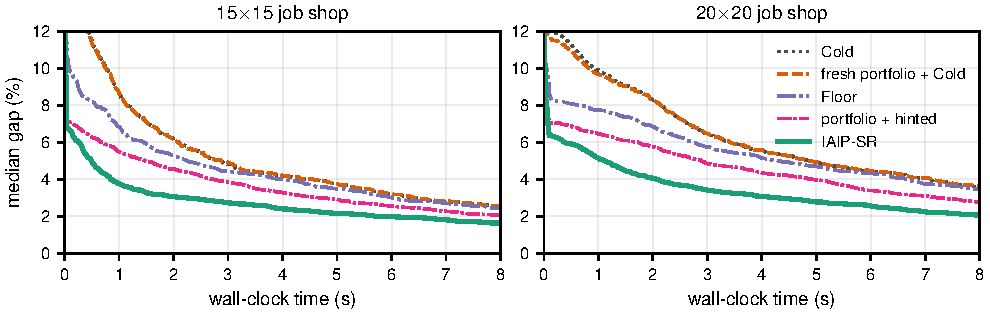
\includegraphics[width=0.95\textwidth]{figures/anytime}
\caption{Median gap to $z^*$ over time on the 1{,}000 confirmatory stream instance runs per size (20 held-out streams $\times$ 10 steps $\times$ 5 solver seeds). The vertical axis is cut at 12\%; every curve is at 100\% before its first schedule.}
\label{fig:anytime}
\end{figure*}

\paragraph{Where the gain comes from.} Adding one component at a time, the mean PI falls from .0597 (\mfresh) to .0495 when history-based members join the portfolio, to .0443 when the continuation is hinted with the resulting incumbent, and to .0339 with the restricted stage. The first and last steps are predeclared comparisons (40/0 streams each); the middle step, not predeclared, is $-10.5$\% (34/6 streams, uncorrected sign test $p=8.4\cdot10^{-6}$). This order-dependent attribution assigns 40\%, 20\% and 40\% of the total reduction to the three components; other orders were not run. Two contrasts locate the effect of the hint. Hinting the continuation with the current, history-informed incumbent helps (\mph{} vs \mpc), whereas hinting it with a fresh dispatching schedule does not (\mfreshh{} vs \mfresh: $+2.5$\%, 13/27 streams, uncorrected $p=0.038$, interval $[-0.0001, 0.0031]$; not predeclared), and Stage~1 showed that hinting with the previous solution or the floor hurts.

\paragraph{Impact-awareness matters.} With a random neighbourhood of the same size, the restricted stage still helps (\mrnd{} .0420 vs \mph{} .0443), but \miaip{} beats it on 36 of 40 streams by 19.4\%. In 1{,}608 of 2{,}000 runs the restricted stage improved the incumbent; in 392 it proved, through the improvement bound, that the neighbourhood contained no better schedule.

\paragraph{By delta type.} Relative to \mfresh{}, \miaip{} reduces PI by 41.7\% after arrivals (38/1 streams), 42.3\% after cancellations (38/0), 47.0\% after duration changes (39/1) and 28.4\% after outages (25/4). The arrival weakness of the floor is gone: after arrivals \mfloor{} (.0650) is worse than \mfresh{} (.0622), \miaip{} is at .0363. Outages are the weakest case; there, hinting the continuation hurts (\mph{} .0469 vs \mpc{} .0443) and the restricted stage only recovers it. These breakdowns are exploratory.

\paragraph{Robustness.} After the confirmatory analysis we specified, and then ran, exploratory experiments with the frozen configuration on 20 new streams per setting and one solver seed (Table~\ref{tab:robust}): budgets of 2 and 30\,s, four CP-SAT workers per run (each process pinned to four physical cores), streams with only arrivals or only outages, high severity, and streams whose base is a published instance (Taillard ta01--ta20 \citep{taillard1993}, dmu01--05 \citep{demirkol1998}, swv01--05 \citep{storer1992}, yn1--4 \citep{yamada1992}; two streams per base, the base instance being the unit). Against \mfresh{} the reduction holds in every setting, and it is \emph{larger} with 30\,s (55.3\%) and with four workers (65.7\%) than in the confirmatory setting, so it is not an artefact of a short single-worker budget. It holds on all 34 published bases. The restricted stage's own contribution, however, depends on the regime: it is large with 30\,s, on arrival-only streams and on published bases, but not detectable at 2\,s (13/7 streams) or with four workers (10/10), where the hinted continuation from the portfolio incumbent already comes close (mean PI .0117 vs .0106). The final gap of \miaip{} is lower than \mfresh's in every setting, with an interval excluding zero in all but the outage-only streams.

\begin{table}[t]
\centering
\small
\setlength{\tabcolsep}{2pt}
\begin{tabular}{lrrrr}
\toprule
Setting & $n$ & vs \mfresh & vs \mph & vs \mfloor \\
\midrule
$B=2$\,s & 20 & $-36$\% 17/3 & $-8$\% 13/7$^\circ$ & $-28$\% 15/5$^\circ$ \\
$B=30$\,s & 20 & $-55$\% 20/0 & $-34$\% 18/2 & $-45$\% 20/0 \\
4 workers & 20 & $-66$\% 20/0 & $-9$\% 10/10$^\circ$ & $-61$\% 20/0 \\
Arrivals only & 20 & $-63$\% 20/0 & $-59$\% 20/0 & $-65$\% 20/0 \\
Outages only & 20 & $-42$\% 18/2 & $-25$\% 17/3 & $-25$\% 16/4 \\
High severity & 20 & $-58$\% 20/0 & $-41$\% 17/3 & $-50$\% 19/1 \\
Publ.\ bases & 34 & $-61$\% 34/0 & $-38$\% 33/1 & $-54$\% 34/0 \\
\bottomrule
\end{tabular}
\caption{Exploratory robustness of the frozen \miaip{} ($B=8$\,s and one worker unless stated). Relative PI difference and W/L of \miaip{} against each method; $n$ streams (published bases: base instances). $^\circ$: not significant (Holm over the four comparisons of each setting, $p\ge 0.05$); all other entries $p\le 0.012$. Every run returned a validated schedule.}
\label{tab:robust}
\end{table}

\paragraph{Comparison with neighbourhood baselines.} Since \miaip's restricted stage is a neighbourhood search, we also compared it with neighbourhood baselines that start from the previous schedule. On 20 further streams (run on different cores, so absolute values are not comparable with the tables above), \miaip{} beat \mfloor{} by 45.0\% (20/0), an LNS that runs 1\,s destroy-and-repair rounds from the previous solution by 84.2\% (20/0), and fix-and-optimize with half the operations fixed by 77.6\% (18/2). These baselines search only within neighbourhoods; \miaip{} makes one restricted solve on the affected region with an improvement bound and then hands the remaining budget to the unrestricted solver. We did not test which of these differences matters.

\section{Limitations}

The confirmatory conclusions are for synthetic full job shops of two sizes, one delta mix, medium severity, one CP-SAT worker and $B=8$\,s; the robustness results for other budgets, four workers, other delta mixes and published bases are exploratory, with one solver seed and 20 streams per setting, and they show that the restricted stage's own contribution is not detectable at 2\,s or with four workers. We did not test more than four workers or budgets beyond 30\,s. $z^*$ is the best value found in each experiment, not a proven optimum. The deltas are randomly generated. Only makespan is optimized. \miaip{} does not constrain how much the schedule changes: on the confirmatory streams it moved 85.9\% of the operations present in consecutive schedules, against 91.1\% for \mfloor{} and 94.7\% for \mcold, so none of the methods is stable in the sense of \citet{fox2006}. The method is specific to job shops: the repair, the disruption set and the neighbourhood would have to be redesigned for other problem classes. The development streams came from the same generator as the held-out streams, so the frozen configuration was selected for this distribution.

\section{Conclusion}

For anytime rescheduling with a constraint solver, how the previous schedule is used matters more than whether it is used. Passed as a hint it hurts; kept as an incumbent it helps, except when the event invalidates its structure. Combining historical and fresh incumbents, a restricted solve around the operations the event affected, and an unrestricted continuation hinted with the current incumbent reduced the primal integral by 43\% against the strongest fresh-incumbent baseline on held-out streams, under a configuration fixed in advance; in exploratory runs the reduction grew with longer budgets and more workers, while the restricted stage itself mattered with one worker and budgets of 8\,s or more but not at 2\,s or with four workers. Fresh-incumbent baselines, not only solving from scratch, are the comparison reuse methods need to beat.

\bibliography{references}

\end{document}
